\usetikzlibrary{math}
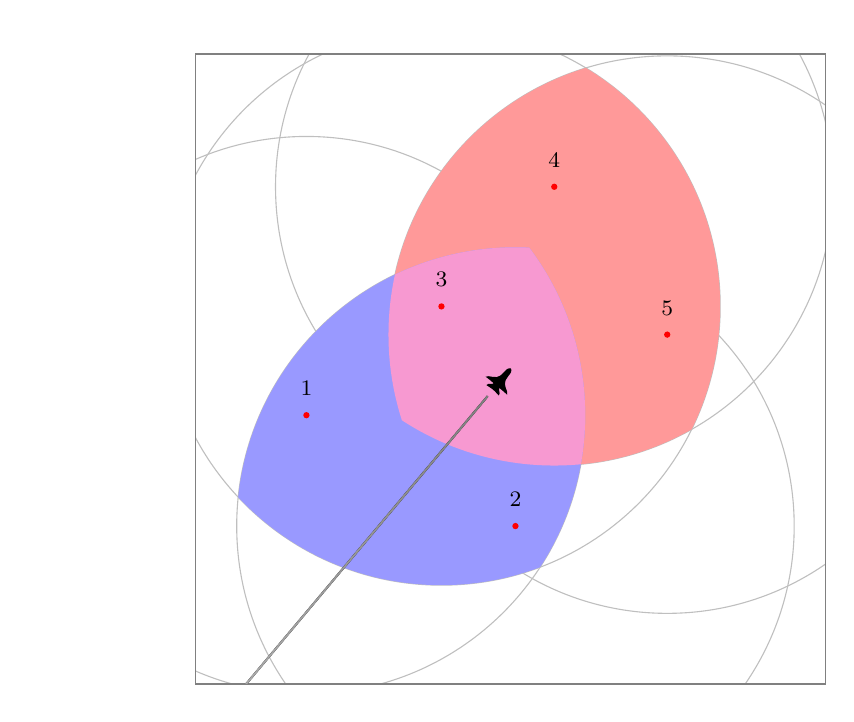
\begin{tikzpicture}[font=\footnotesize]

% Sizes
\tikzmath{\srange = 3.54; \sradius = 0.04;}

% Sensor locations (sensor 3 is shared)
\coordinate (s1) at (1.4086,-4.5869);
\coordinate (s2) at (4.0633,-5.9948);
\coordinate (s3) at (3.1235,-3.2054);
\coordinate (s4) at (4.5563,-1.6861);
\coordinate (s5) at (5.9909,-3.5635);

% Navigator location
\coordinate (nav_loc) at (4,-4);

% Bounding rectangle
\coordinate (brect_start) at (0,0);
\coordinate (brect_end) at (8.0, -8.0);


% Gray range circles
\begin{scope}
\clip (brect_start) rectangle (brect_end);
\draw[gray!50] (s1) circle (\srange);
\draw[gray!50] (s2) circle (\srange);
\draw[gray!50] (s3) circle (\srange);
\draw[gray!50] (s4) circle (\srange);
\draw[gray!50] (s5) circle (\srange);
\end{scope}

% Red subgroup overlap
\begin{scope}
\clip (s3) circle (\srange);
\clip (s4) circle (\srange);
\clip (s5) circle (\srange);
\fill[red!40] (brect_start) rectangle (brect_end);
\end{scope}

% Blue subgroup overlap
\begin{scope}
\clip (s1) circle (\srange);
\clip (s2) circle (\srange);
\clip (s3) circle (\srange);
\fill[blue!40] (brect_start) rectangle (brect_end);
\end{scope}

% Magenta double overlap
\begin{scope}
\clip (s1) circle (\srange);
\clip (s2) circle (\srange);
\clip (s3) circle (\srange);
\clip (s4) circle (\srange);
\clip (s5) circle (\srange);
\fill[magenta!40] (brect_start) rectangle (brect_end);
\end{scope}

% Sensors
\fill[red] (s1) circle (\sradius);
\fill[red] (s2) circle (\sradius);
\fill[red] (s3) circle (\sradius);
\fill[red] (s4) circle (\sradius);
\fill[red] (s5) circle (\sradius);

% Bounding box
\draw[gray] (brect_start) rectangle (brect_end);

% Navigator
\clip (brect_start) rectangle (brect_end);
\begin{scope}[shift={(nav_loc)},rotate=-40,xscale=0.25,yscale=0.3]
% Plane
\draw[fill]  plot[smooth, tension=.6] coordinates {
(-0.65,-0.9) 
(-0.6,-0.85) 
(-0.4,-0.75) 
(-0.25,-0.65) 
(-0.15,-0.5) 
(-0.12,-0.3) 
(-0.10,-0.1) 
(0.0,0.0) 
(0.10,-0.1) 
(0.12,-0.3) 
(0.15,-0.5) 
(0.25,-0.65) 
(0.4,-0.75) 
(0.6,-0.85) 
(0.65,-0.9)
} -- plot[smooth, tension=.6] coordinates {
(0.65,-0.9) 
(0.15,-0.91)
(0.35,-1.1) 
(0.37,-1.15)
} -- plot[smooth, tension=.6] coordinates {
(0.37,-1.15)
(0.0,-1.12) 
(-0.37,-1.15) 
} -- plot[smooth, tension=.6] coordinates {
(-0.37,-1.15)
(-0.35,-1.1) 
(-0.15,-0.91) 
(-0.65,-0.9) 
} -- cycle;
% Trail
\fill[bottom color=white, top color=gray] (-0.05, -1.5) rectangle (0.05, -50);
\end{scope}
\node[label=1] at (s1) {};
\node[label=2] at (s2) {};
\node[label=3] at (s3) {};
\node[label=4] at (s4) {};
\node[label=5] at (s5) {};
\end{tikzpicture}













